\documentclass{beamer}
\usepackage{graphicx, parskip, microtype}

\frenchspacing

\usetheme{default}
\usecolortheme{orchid}

\title{(Mis)information visualization}
\author{Peter D Smits}
\institute{Committee on Evolutionary Biology \\
University of Chicago}
\date{\today}

\AtBeginSection[]
{
  \begin{frame}
    \frametitle{Outline}
    \tableofcontents[currentsection]
  \end{frame}
}

\begin{document}

\begin{frame}
  \maketitle
\end{frame}

\begin{frame}
  \frametitle{Outline}
  \tableofcontents
\end{frame}

\section{Good data visualization}
\begin{frame}
  \frametitle{Minard's depiction of Napoleon's invasion of Russia}
  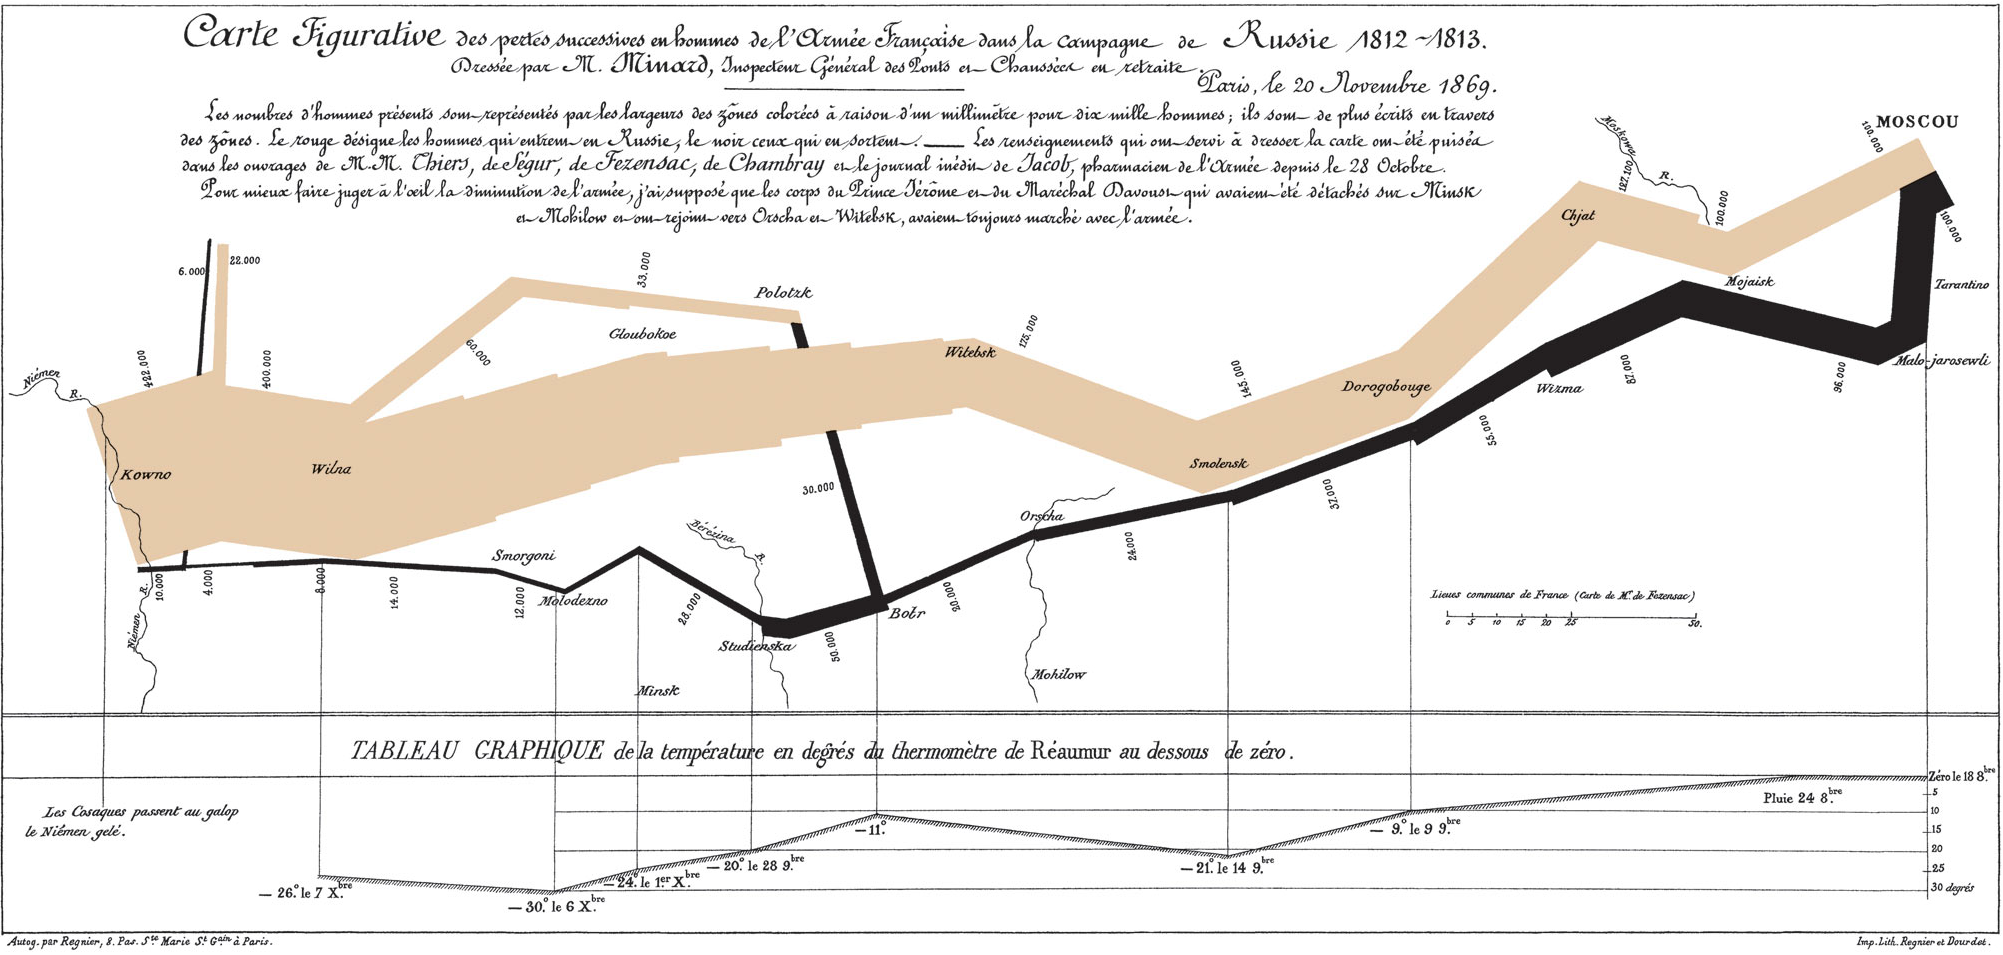
\includegraphics[width = \textwidth, keepaspectratio = true]{figure/minard}
\end{frame}

\begin{frame}
  \frametitle{Beautiful}
  \begin{center}
    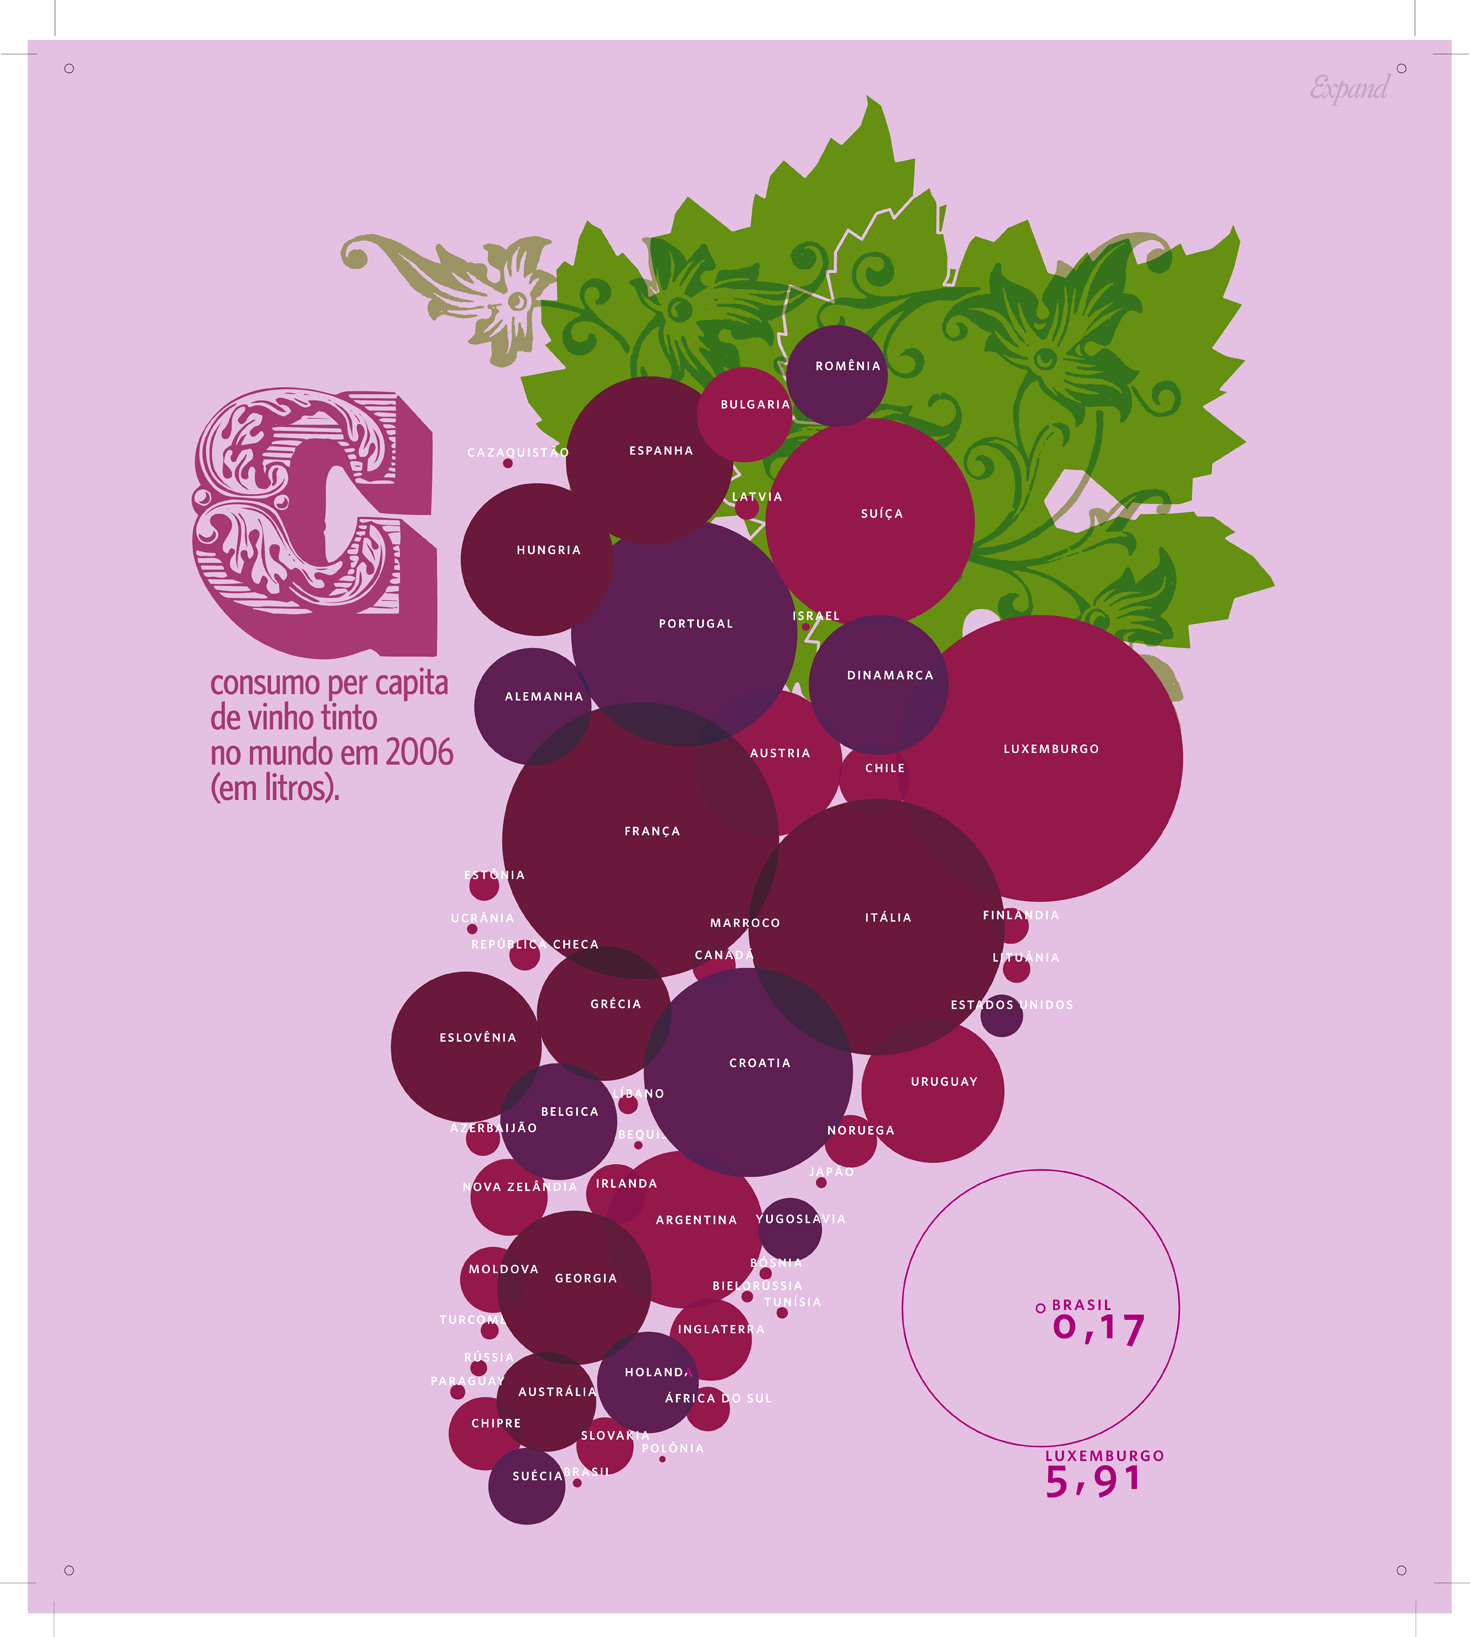
\includegraphics[height = 0.9\textheight, keepaspectratio = true]{figure/wine_consumption_2006}
  \end{center}
\end{frame}

\begin{frame}
  \frametitle{Tells a story}
  \begin{center}
    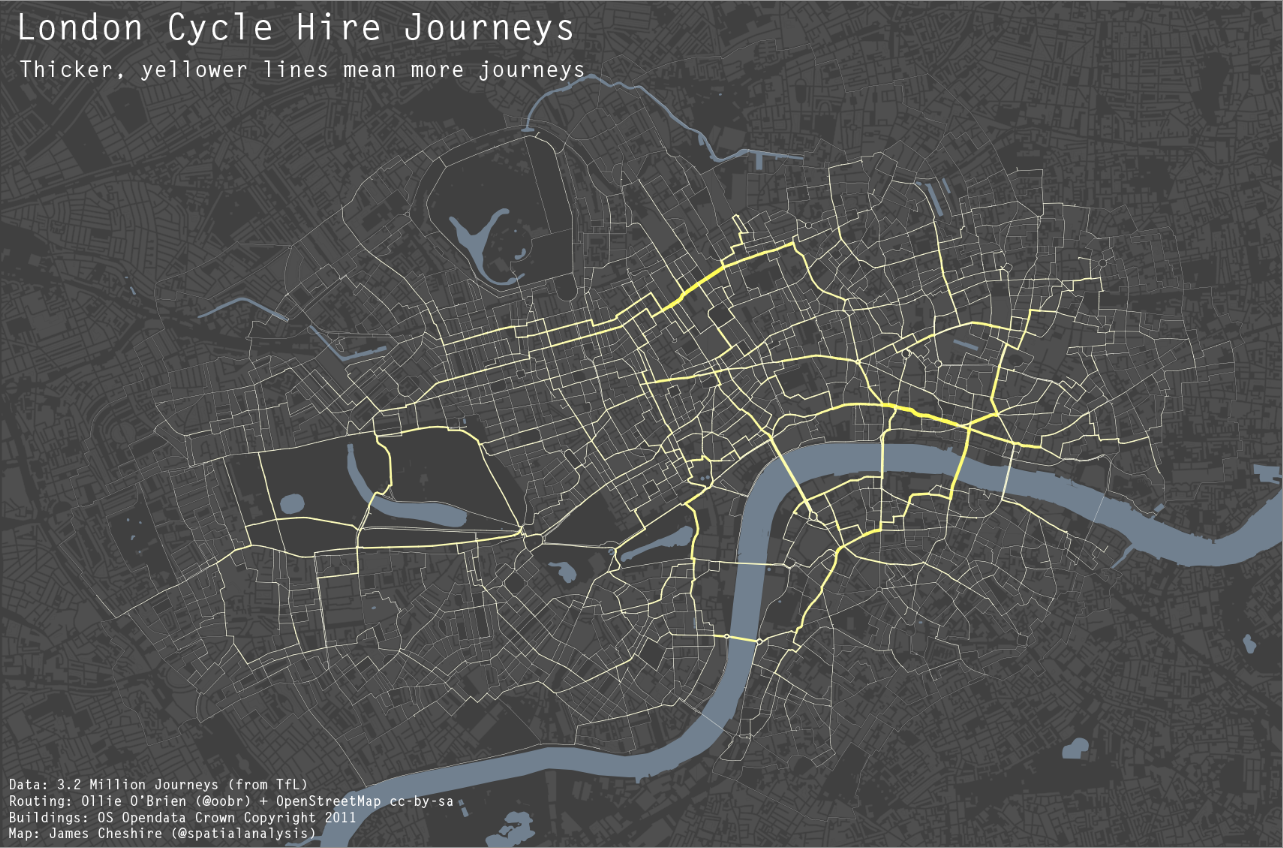
\includegraphics[width = \textwidth, keepaspectratio = true]{figure/bike_ggplot}
  \end{center}
\end{frame}

\begin{frame}
  \frametitle{Gives advice}
  \begin{center}
    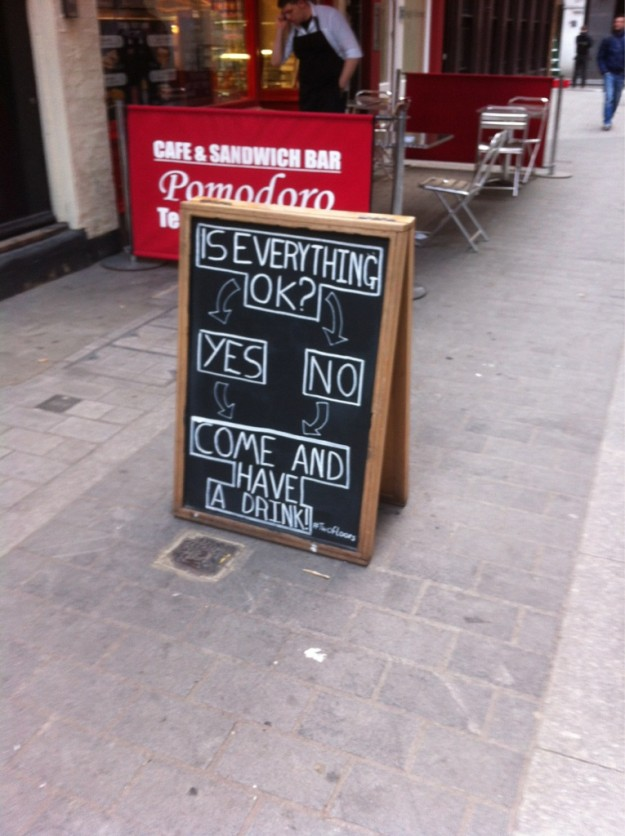
\includegraphics[height = 0.8\textheight, keepaspectratio = true]{figure/pub_flow}
  \end{center}
\end{frame}


\section{Academic}
% need citations
\begin{frame}
  \frametitle{;\_;}
  \begin{center}
    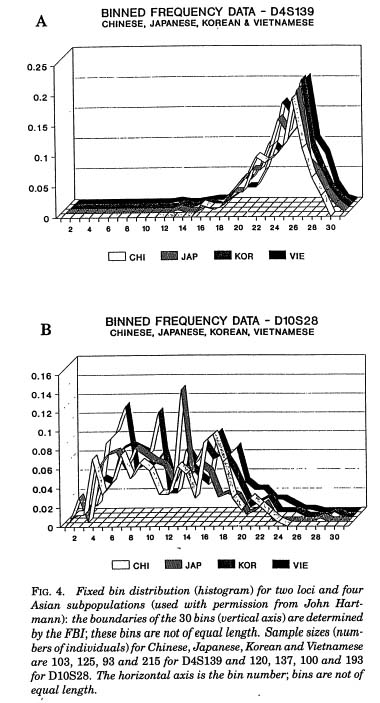
\includegraphics[height = 0.8\textheight, keepaspectratio = true]{figure/roeder_fig4}
  \end{center}
\end{frame}

\begin{frame}
  % straight line
  \frametitle{These say what exactly?}
  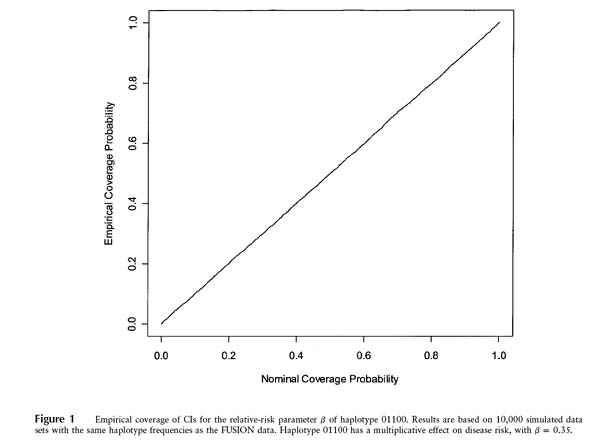
\includegraphics[width = \textwidth, keepaspectratio = true]{figure/epstein_fig1}
\end{frame}

\begin{frame}
  \frametitle{Surely that was a unique phenomenon\ldots}
  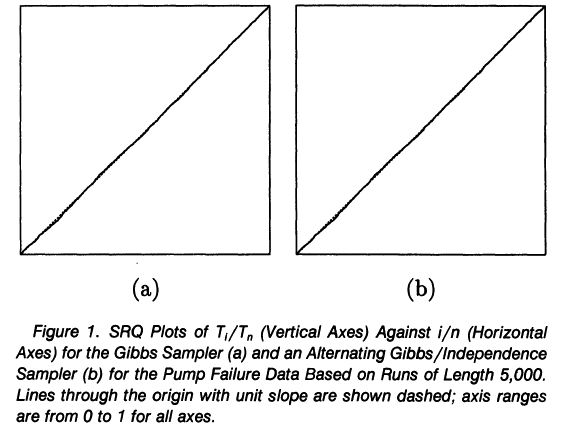
\includegraphics[width = \textwidth, keepaspectratio = true]{figure/mykland_fig1}
\end{frame}

\begin{frame}
  % 3d pie chart
  \frametitle{What is worse than one pie chart?}
  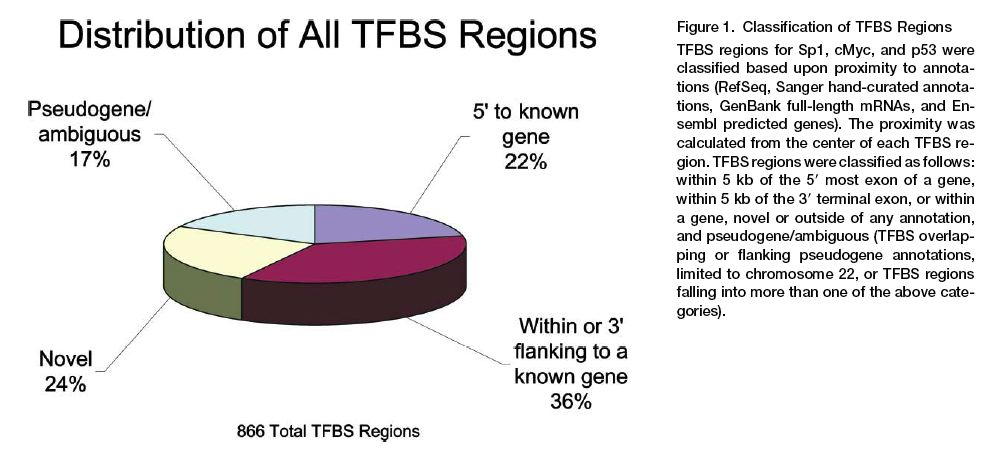
\includegraphics[width = \textwidth, keepaspectratio = true]{figure/cawley_fig1}
\end{frame}

\begin{frame}
  % 9 pie charts!
  \frametitle{Can it even get worse?}
  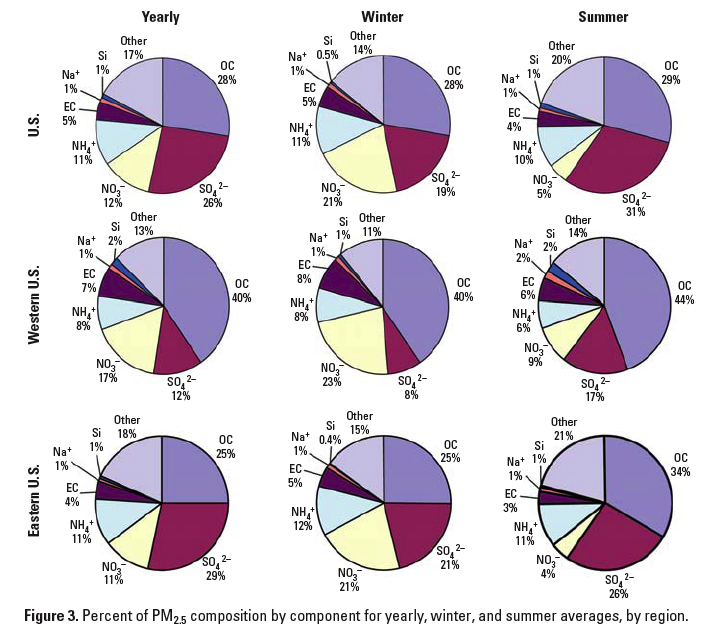
\includegraphics[height = 0.8\textheight, keepaspectratio = true]{figure/bell_fig3}
\end{frame}

\begin{frame}
  \frametitle{Pardon me as I vomit}
  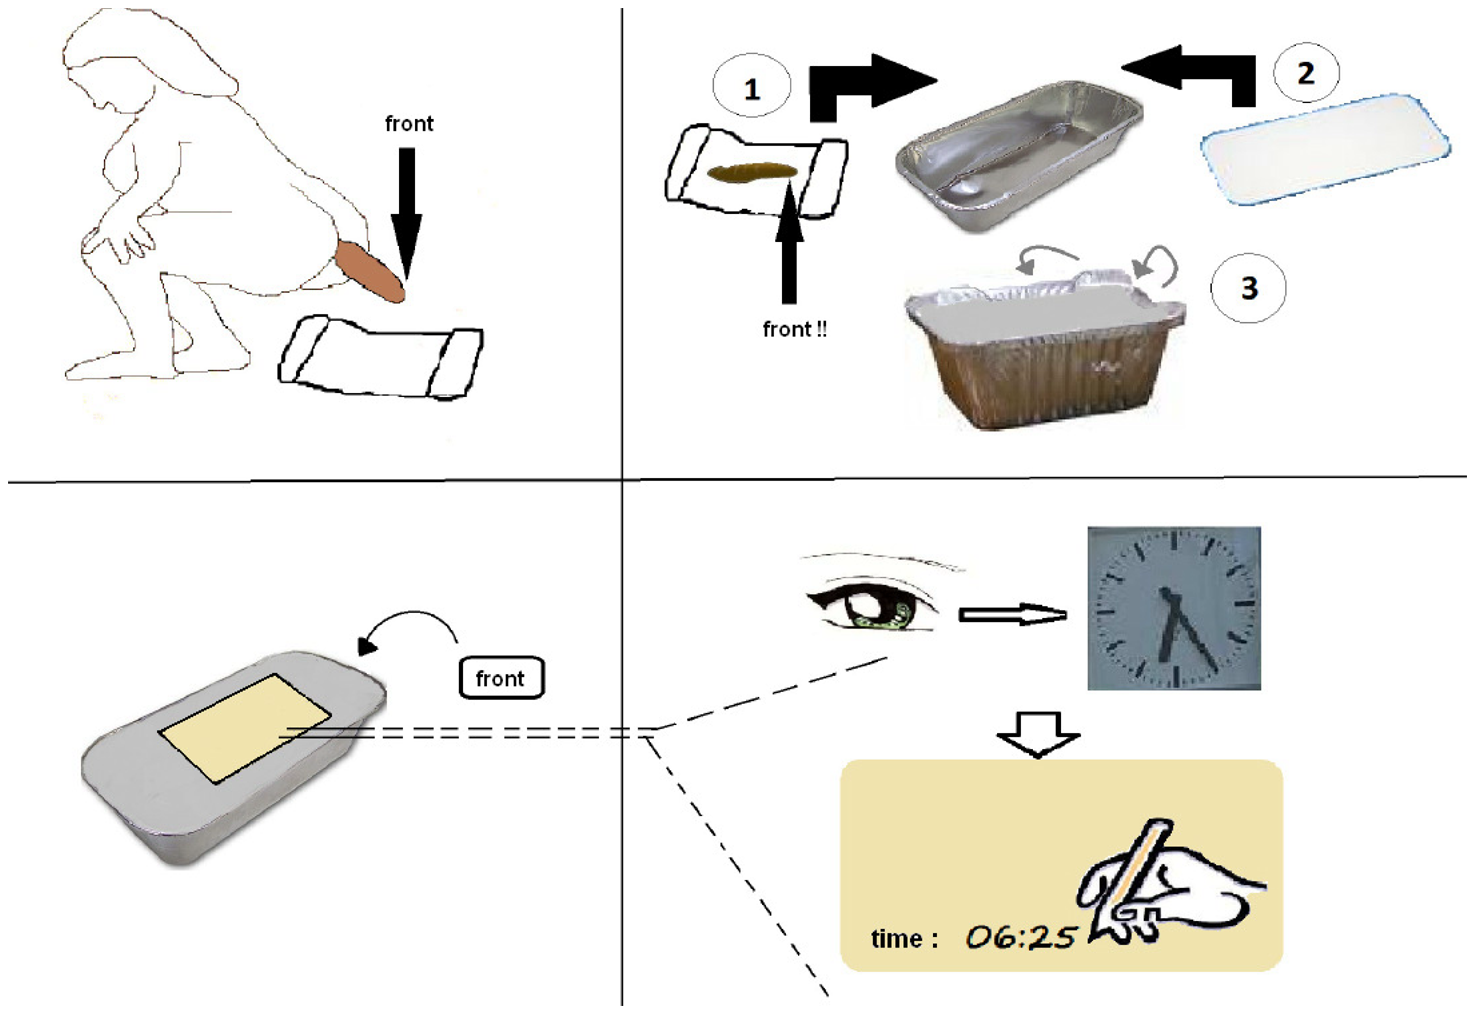
\includegraphics[width = \textwidth, keepaspectratio = true]{figure/poop}
\end{frame}

\begin{frame}
  
\includegraphics[width = \textwidth, keepaspectratio = true]{figure/nerd_shit}
\end{frame}

\section{Media}
\begin{frame}
  \frametitle{Wrong choice}
  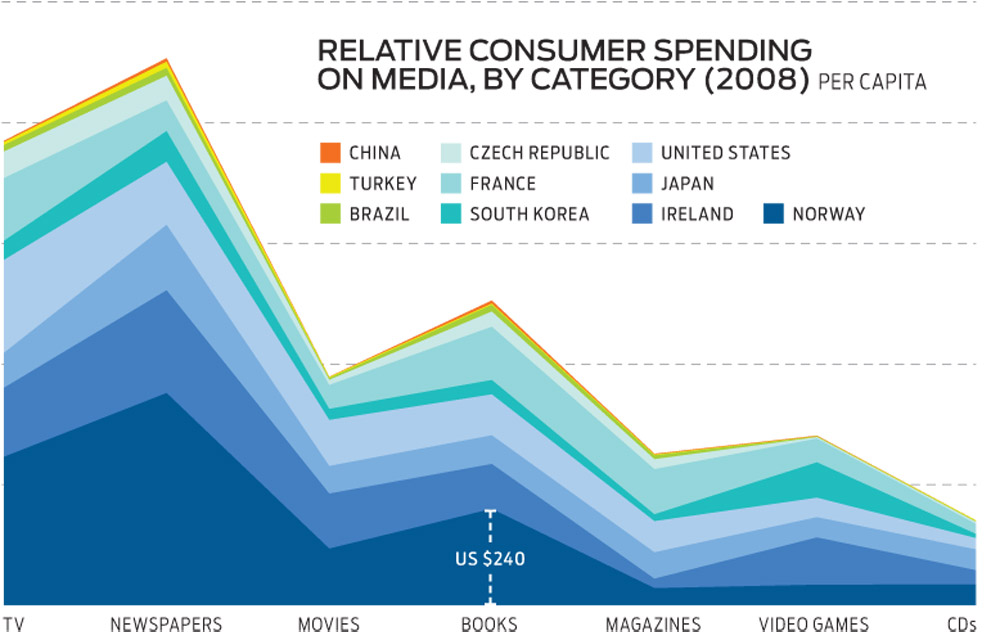
\includegraphics[width = \textwidth, keepaspectratio = true]{figure/not_lines}
\end{frame}

\begin{frame}
  \frametitle{My sides}
  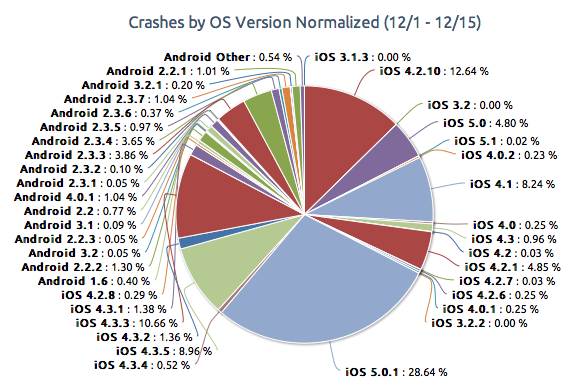
\includegraphics[width = \textwidth, keepaspectratio = true]{figure/android}
\end{frame}

\begin{frame}
  \frametitle{Does this even mean anything?}
  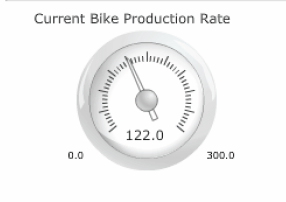
\includegraphics[width = \textwidth, keepaspectratio = true]{figure/gauge1}
\end{frame}

\begin{frame}
  \frametitle{Why can't I hold all these graphical sins?}
  \begin{center}
    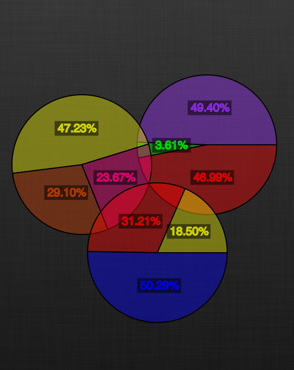
\includegraphics[height = 0.8\textheight, keepaspectratio = true]{figure/pie-agram}
  \end{center}
\end{frame}

\begin{frame}
  \frametitle{What is this I don't even}
  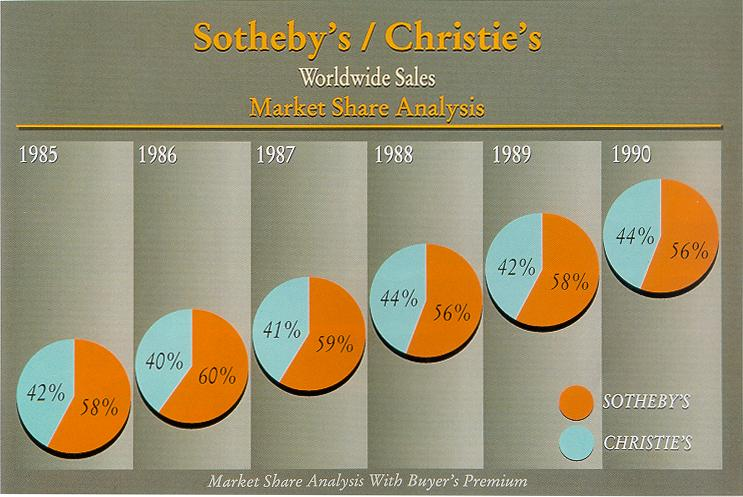
\includegraphics[width = \textwidth, keepaspectratio = true]{figure/sothebys}
\end{frame}

\begin{frame}
  \frametitle{Oh god how did this get here I am not good with questions}
  \begin{center}
    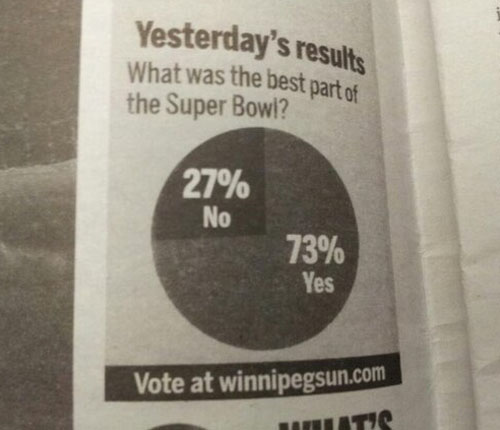
\includegraphics[height = 0.8\textheight, keepaspectratio = true]{figure/super_bowl}
  \end{center}
\end{frame}

\begin{frame}
  \frametitle{Fox is an easy target}
  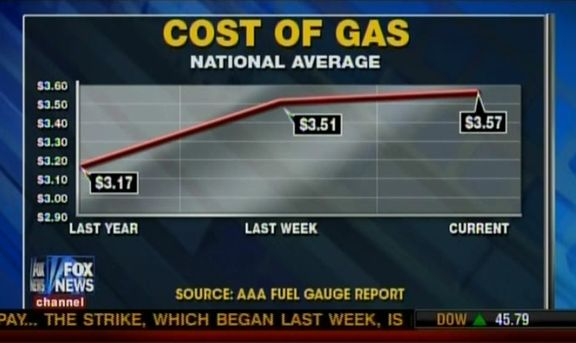
\includegraphics[width = \textwidth, keepaspectratio = true]{figure/fox_scale}
\end{frame}

\begin{frame}
  \frametitle{A really easy target\ldots}
  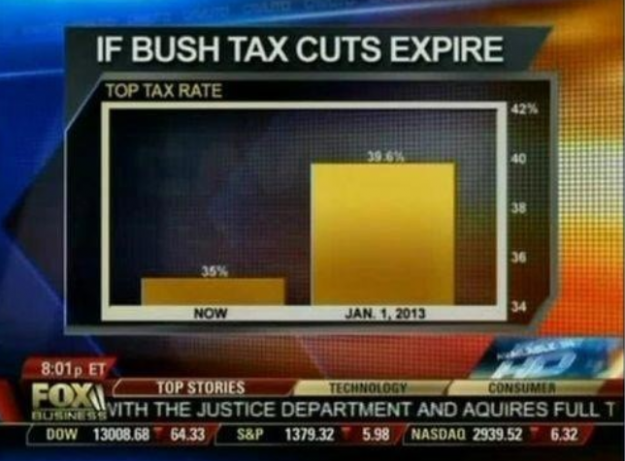
\includegraphics[width = \textwidth, keepaspectratio = true]{figure/fox_nodiff}
\end{frame}

\begin{frame}
  \frametitle{Too easy even}
  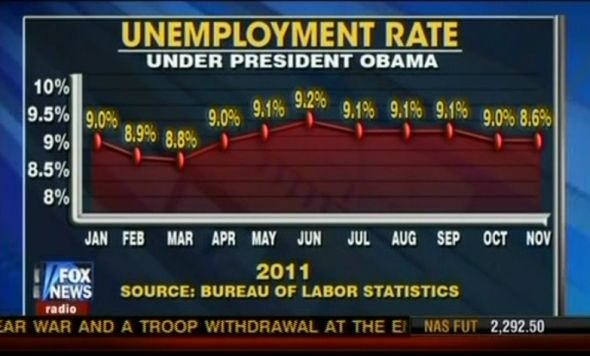
\includegraphics[width = \textwidth, keepaspectratio = true]{figure/fox_lying}
\end{frame}

\begin{frame}
  \frametitle{{[}Screams internally{]}}
  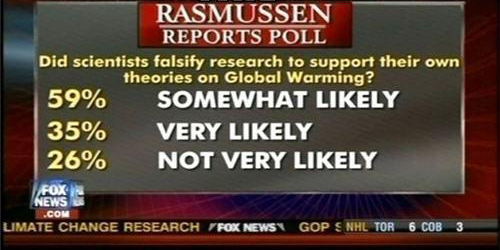
\includegraphics[width = \textwidth, keepaspectratio = true]{figure/fox_warming}
\end{frame}

\begin{frame}
  \frametitle{They can't even get the worst graph ``right''\ldots}
  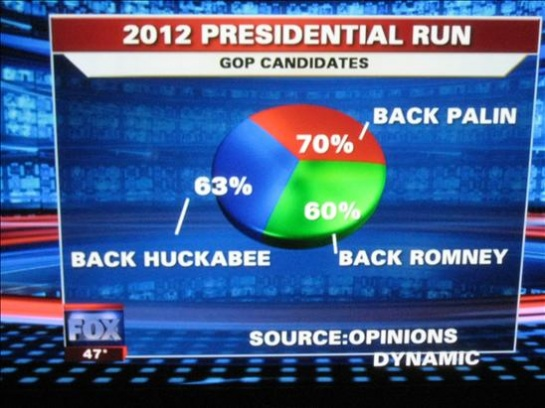
\includegraphics[width = \textwidth, keepaspectratio = true]{figure/fox-news-piechart}
\end{frame}



\section{Excel}
\begin{frame}
  \frametitle{3D is best D}
  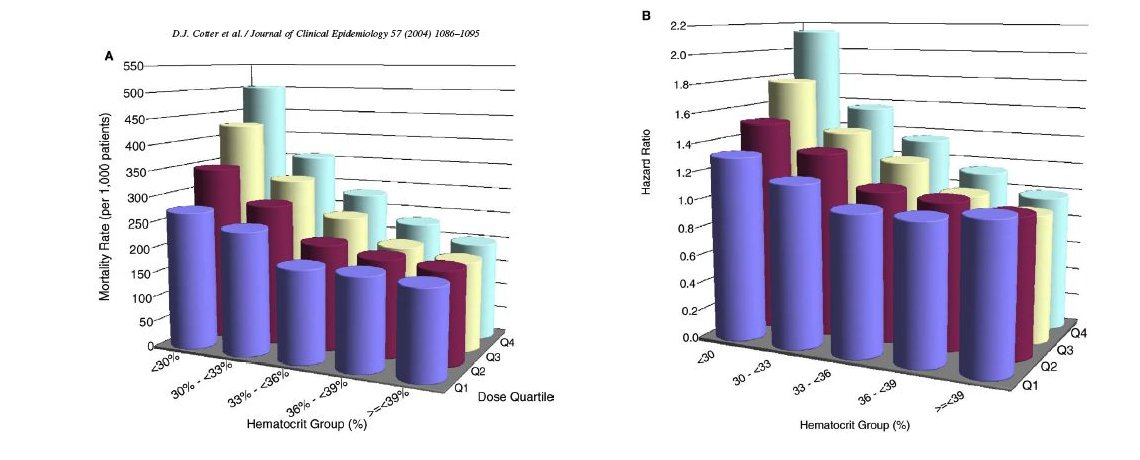
\includegraphics[width = \textwidth, keepaspectratio = true]{figure/cotter_fig2}
\end{frame}

\begin{frame}
  \frametitle{Absolute best D}
  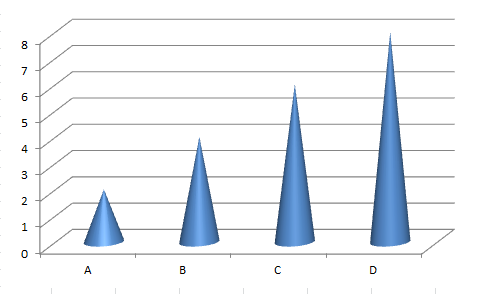
\includegraphics[width = \textwidth, keepaspectratio = true]{figure/cones}
\end{frame}

\begin{frame}
  \frametitle{I'm embarrassed}
  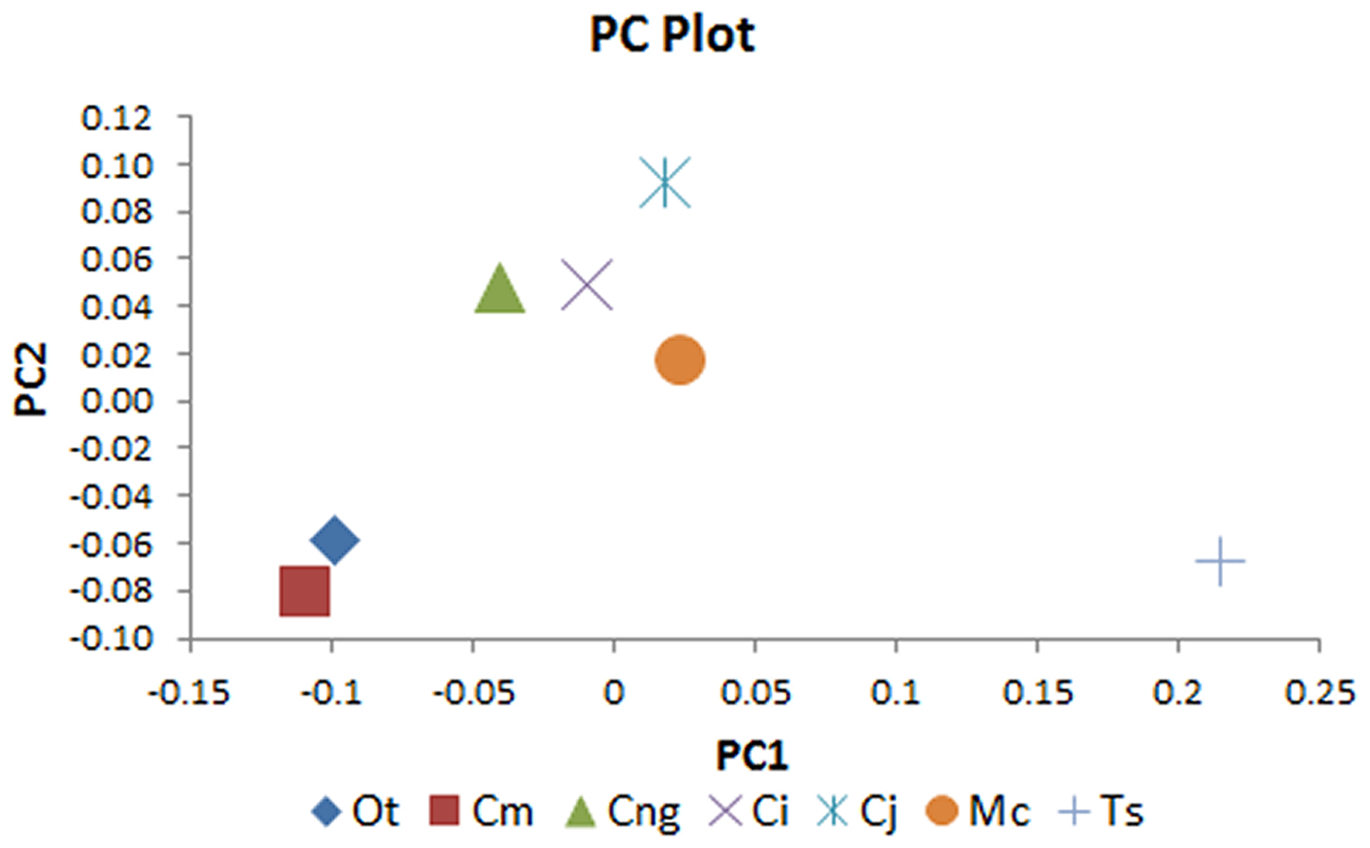
\includegraphics[width = \textwidth, keepaspectratio = true]{figure/wamsley_pca}
\end{frame}

\begin{frame}
  \frametitle{Really embarrassed}
  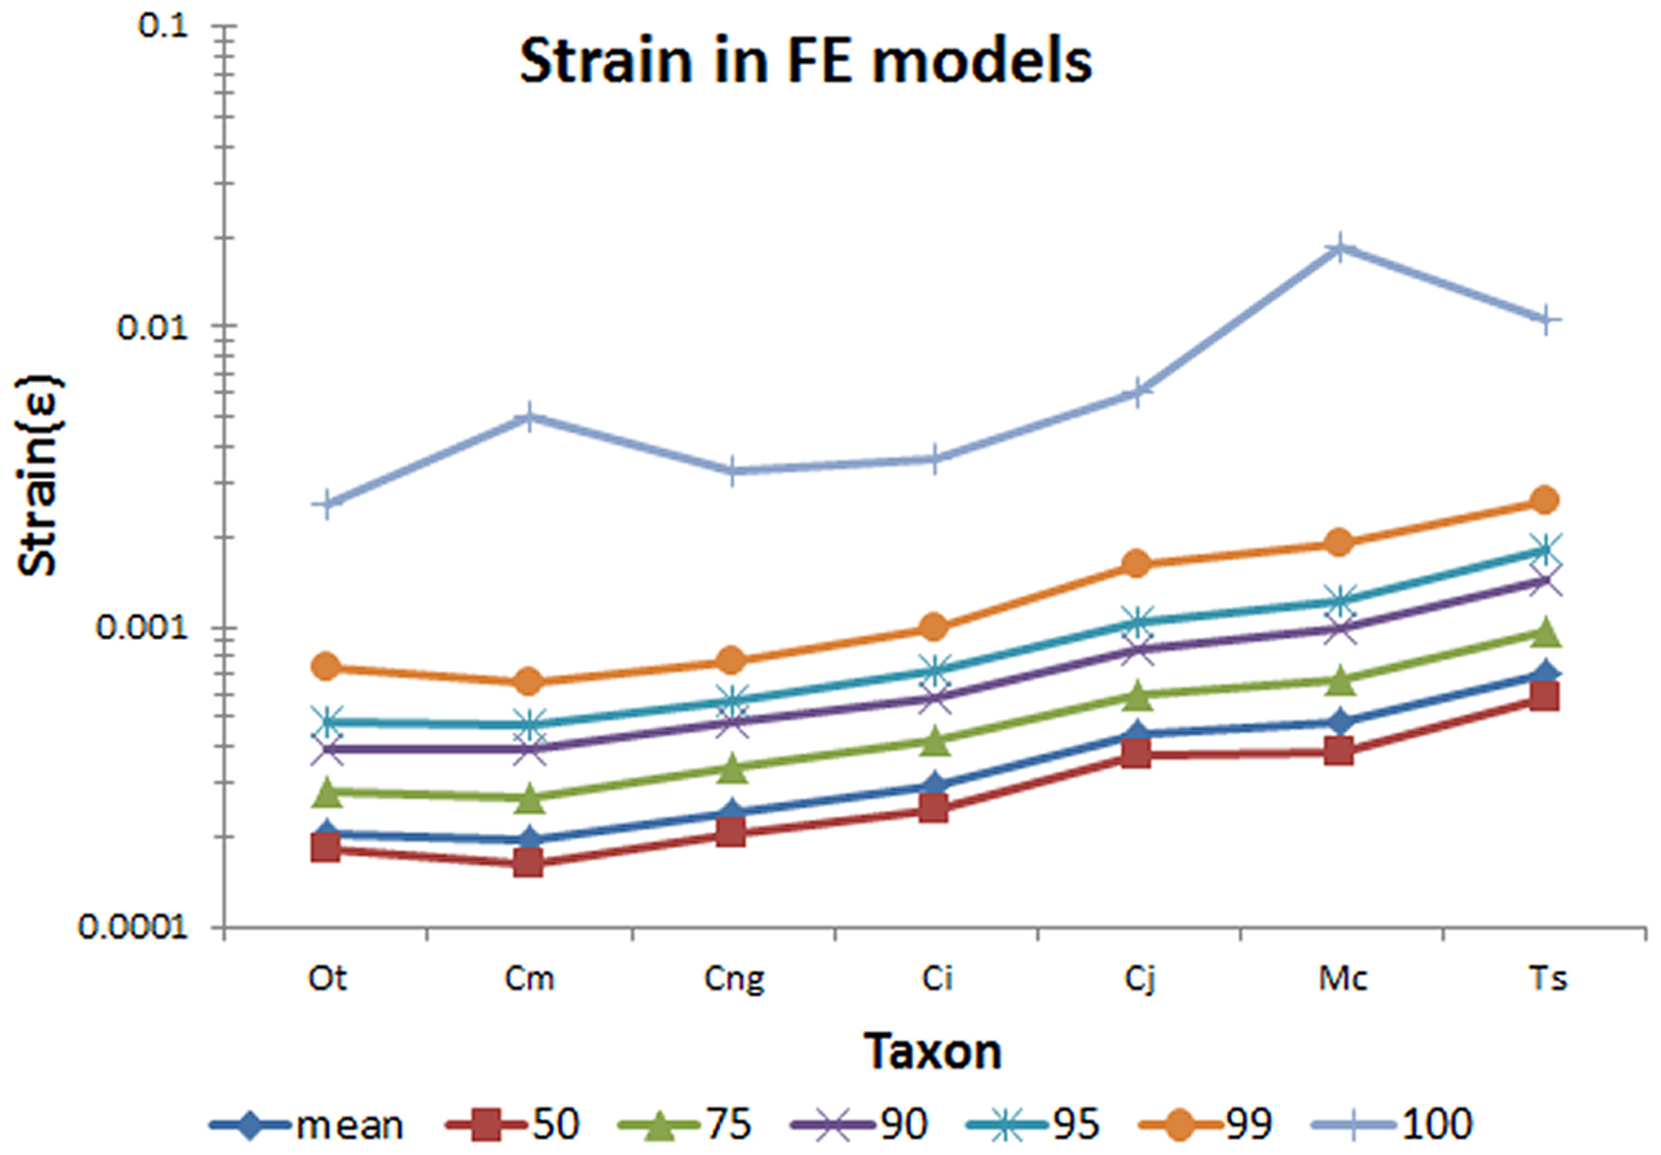
\includegraphics[height = 0.8\textheight, keepaspectratio = true]{figure/wamsley_line}
\end{frame}

\section{Things to remember}
\begin{frame}
  \begin{center}
    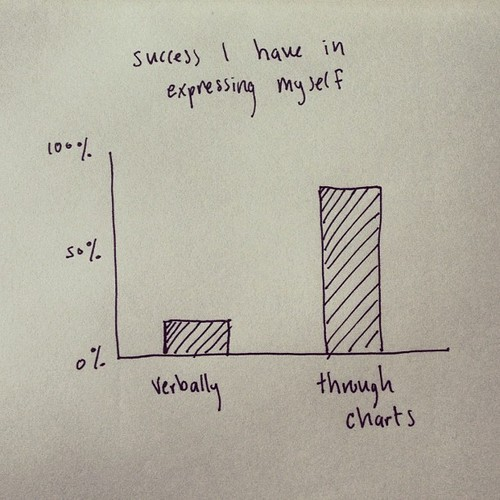
\includegraphics[height = \textheight, keepaspectratio = true]{figure/success}
  \end{center}
\end{frame}

\begin{frame}
  \begin{center}
    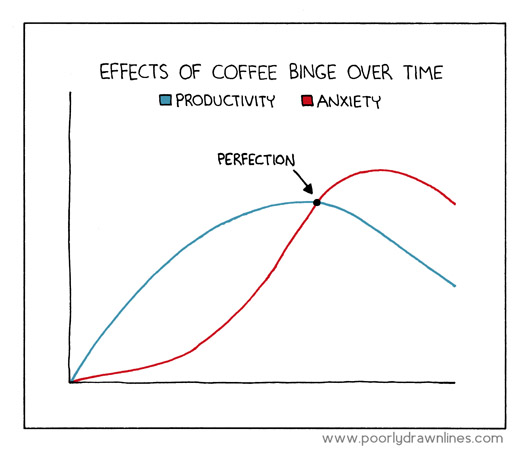
\includegraphics[height = 0.8\textheight, keepaspectratio = true]{figure/coffee-binge}
  \end{center}
\end{frame}

\begin{frame}
  \begin{center}
    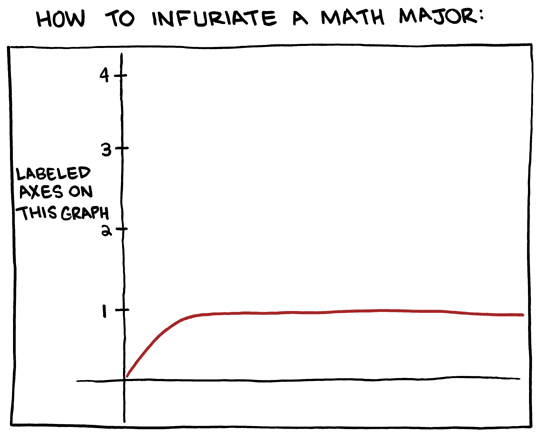
\includegraphics[height = 0.8\textheight, keepaspectratio = true]{figure/trick}
  \end{center}
\end{frame}

\begin{frame}
  \begin{center}
    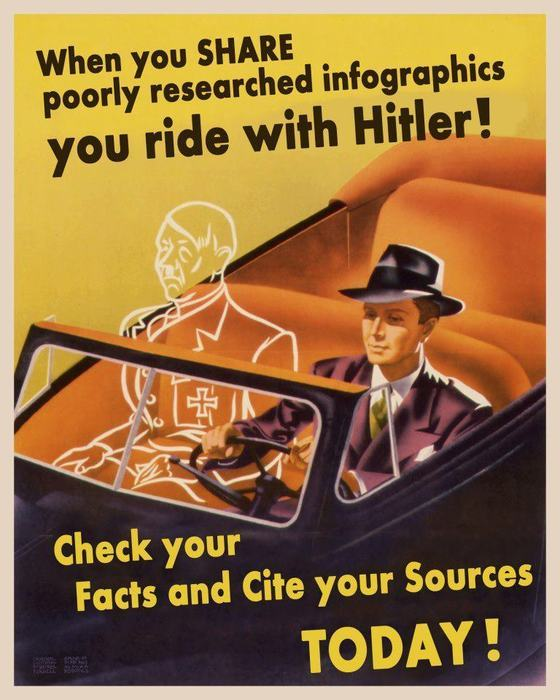
\includegraphics[height = \textheight, keepaspectration = true]{figure/ride_hitler}
  \end{center}
\end{frame}

\begin{frame}
  \begin{center}
    \frametitle{I'm 12 and what is this?}
    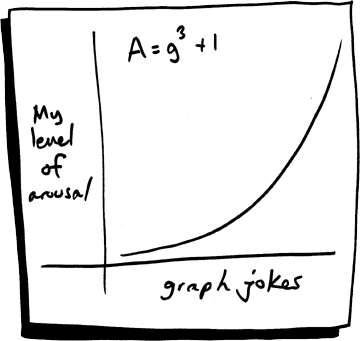
\includegraphics[height = 0.8\textheight, keepaspectration = true]{figure/graph_smbc}
  \end{center}
\end{frame}


\end{document}
